\documentclass[10pt, conference, letterpaper]{IEEEtran}

\usepackage{algorithm}
\usepackage{algorithmicx}
\usepackage{algpseudocode}
\usepackage{amsfonts}
\usepackage{amsmath}
\usepackage{amssymb}
\usepackage[ansinew]{inputenc}
\usepackage{xcolor}
\usepackage{mathtools}
\usepackage{graphicx}
\usepackage{caption}
\usepackage{subcaption}
\usepackage{import}
\usepackage{multirow}
\usepackage{cite}
\usepackage[export]{adjustbox}
\usepackage{breqn}
\usepackage{mathrsfs}
\usepackage{acronym}
%\usepackage[keeplastbox]{flushend}
\usepackage{setspace}
\usepackage{bm}
\usepackage{stackengine}

\usepackage{listings}

\lstset{%
 backgroundcolor=\color[gray]{.85},
 basicstyle=\small\ttfamily,
 breaklines = true,
 keywordstyle=\color{red!75},
 columns=fullflexible,
}%

\lstdefinelanguage{BibTeX}
  {keywords={%
      @article,@book,@collectedbook,@conference,@electronic,@ieeetranbstctl,%
      @inbook,@incollectedbook,@incollection,@injournal,@inproceedings,%
      @manual,@mastersthesis,@misc,@patent,@periodical,@phdthesis,@preamble,%
      @proceedings,@standard,@string,@techreport,@unpublished%
      },
   comment=[l][\itshape]{@comment},
   sensitive=false,
  }

\usepackage{listings}

% listings settings from classicthesis package by
% Andr\'{e} Miede
\lstset{language=[LaTeX]Tex,%C++,
    keywordstyle=\color{RoyalBlue},%\bfseries,
    basicstyle=\small\ttfamily,
    %identifierstyle=\color{NavyBlue},
    commentstyle=\color{Green}\ttfamily,
    stringstyle=\rmfamily,
    numbers=none,%left,%
    numberstyle=\scriptsize,%\tiny
    stepnumber=5,
    numbersep=8pt,
    showstringspaces=false,
    breaklines=true,
    frameround=ftff,
    frame=single
    %frame=L
}

\renewcommand{\thetable}{\arabic{table}}
\renewcommand{\thesubtable}{\alph{subtable}}

\DeclareMathOperator*{\argmin}{arg\,min}
\DeclareMathOperator*{\argmax}{arg\,max}

\def\delequal{\mathrel{\ensurestackMath{\stackon[1pt]{=}{\scriptscriptstyle\Delta}}}}

\graphicspath{{./figures/}}
\setlength{\belowcaptionskip}{0mm}
\setlength{\textfloatsep}{8pt}

\newcommand{\eq}[1]{Eq.~\eqref{#1}}
\newcommand{\fig}[1]{Fig.~\ref{#1}}
\newcommand{\tab}[1]{Tab.~\ref{#1}}
\newcommand{\secref}[1]{Section~\ref{#1}}

\newcommand\MR[1]{\textcolor{blue}{#1}}
\newcommand\red[1]{\textcolor{red}{#1}}
\newcommand{\mytexttilde}{{\raise.17ex\hbox{$\scriptstyle\mathtt{\sim}$}}}

%\renewcommand{\baselinestretch}{0.98}
% \renewcommand{\bottomfraction}{0.8}
% \setlength{\abovecaptionskip}{0pt}
\setlength{\columnsep}{0.2in}

% \IEEEoverridecommandlockouts\IEEEpubid{\makebox[\columnwidth]{PUT COPYRIGHT NOTICE HERE \hfill} \hspace{\columnsep}\makebox[\columnwidth]{ }}

\title{Devices Heterogeneities: augmenting CNN with autoencoder features to prevent HAR imbalance}

\title{Using CNN with autoencoder features for Human Activity Recognition in real use case scenarios}

\author{Bryan Lucchetta$^\dag$, Luca Parolari$^\dag$
\thanks{$^\dag$Department of Mathematics, University of Padova, email: \{bryan.lucchetta, luca.parolari\}@studenti.unipd.it}
}

\IEEEoverridecommandlockouts

\newcounter{remark}[section]
\newenvironment{remark}[1][]{\refstepcounter{remark}\par\medskip
   \textbf{Remark~\thesection.\theremark. #1} \rmfamily}{\medskip}

\begin{document}

\maketitle

\begin{abstract}
Using smartphones sensors for predicting the current activity performed by a user could be a very useful feature for most of fitness mobile apps out there. However, when dealing with cheap sensors and real use case scenarios, this task can easily become very challenging. A key question in particular is how to mitigate Human Activity Recognition (HAR) impairments in every day life smartphone usage. In this paper, we study the effects of smartphones' heterogeneity in state-of-the-art models, and propose solutions such as Orientation Independent Transform preprocessing techniques to mitigate them. Furthermore we investigate the benefits of combining automatic autoencoder extracted features in the best known model in literature nowadays, base upon Convolutional Neural Network (CNN). We then first test our architecture on Heterogeneity Dataset outperforming previous obtained results, and then test it on a new real use case collected dataset, obtaining in this case promising results. \\
\end{abstract}

\IEEEkeywords
Mobile Sensing, Human Activity Recognition, Convolutional Neaural Networks, Autoencoders
\endIEEEkeywords


% !TEX root = template.tex

\section{Introduction}
\label{sec:introduction}

Recognition of the activity that a user is currently doing is
important not only for health care monitoring or security concerns,
but also for developing mobile apps that are able to use this
information to improve our day life.

Developing mobile apps that are capable to track user activities \textit{``in-the-wild''} contexts leads relevant challenges that need to be tackle
down. As stated in \cite{blunck2013heterogeneity} many variables are
involved both coming from users and smartphones. Users are
demographically different (age, stature, weight, ...) and perform
activities in different ways, using their device in their own
style. Devices instead, share among them different operating-systems,
hardware and sensing capabilities.

In a recent work by K. Chen et al. \cite{chen2020deep}, the authors analyze state-of-the-art
deep learning methods for sensor-based HAR, highlighting challenges for HAR tasks, based on their reasons and analyze how existing deep
methods are adopted to address novel challenges. Some of these
includes for example, recognizing concurrent and composite activities
and dealing with scarse annotated, class imbalanced and scarse user
distributed datasets.

In this paper we try to perform HAR with smartphone sensors in real
use case scenarios, where mobile phones can be hold inside trousers
pockets or in a pouch with different orientations, or more simply in a
hand. This is particularly relevant when developing mobile apps
capable of performing HAR, to improve users quality of life. We
propose a CNN architecture augmented with features extracted from an
autoencoder, and then compare the results with other
works. Furthermore we investigate the main benefits of a well thought-out
pre-processing pipeline, like orientation independent transformation
block that remove the HAR impairments when smartphone are used in
different orientation and positions. With this work we aim to study
heterogeneity impairments in real use case scenarios using previous
state-of-the-art models, and then proposed a novel learning framework
that can be used in developing mobile apps for HAR tasks.

Our main contributions can be summarized as follows.

\begin{itemize}
  \item We propose an architecture that combines CNN and automatic
    feature extraction to perform HAR. In particular, augmenting a
    traditional CNN model with autoencoder's features rather than
    manual features can lead to better results.
  \item We study the importance of a good preprocessing pipeline, to
    mitigate heterogeneity when dealing with multiple types of
    smartphones. Also, orientation independent transformation can give
    promising results in real use case scenarios where smartphones can
    be in any position and orientation.
  \item We show that good results can be obtained
    w.r.t. state-of-the-art works also when few computational
    resources are available, i.e, smartphones.
\end{itemize}

This paper is structured as follows. In Section \ref{sec:related-work}
we describe the state-of-the-art, the system and data models are
respectively presented in Sections \ref{sec:processing-pipeline} and
\ref{sec:signals-and-features}. The proposed signal processing
technique is detailed in Section \ref{sec:learning-framework} and its
performance evaluation is carried out in Section
\ref{sec:results}. Concluding remarks are provided in Section
\ref{sec:concluding-remarks}.

%Conclusions:  So to mitigate all these problem when developing Human Activity Recognition (HAR) Systems a representative dataset of all the possibly end-users of out mobile app is required and other pre-processing technique are required for mitigating the heterogenity among devices.


% !TEX root = template.tex

\section{Related Work}
\label{sec:related-work}

HAR is a very wide discipline full of pitfalls and problems. For
example, K. Chen et al. in \cite{chen2020deep} studied HAR in the
broad sense with an eye on it's challenges starting from feature
extraction up to class imbalance, computational cost and many
more. Instead, A. Stisen et al. in \cite{stisen2015smart} studied the
technical details and problems due to heterogeneity among users,
sensors and environemnt. This heterogeneity, as they say, leads to
very low performances when models trained in controlled environment
are brought in real scenario.

One of this state-of-the-art model is presented in
\cite{ignatov2018real} where A. Ignativ uses a Convolutional Neural
Network for local feature extraction together with simple statistical
features for preserving information about the global form of time
series. They also investigate the impact of time series length on the
recognition accuracy. The accuracy of the proposed approach is
evaluated on two commonly used WISDM and UCI datasets that contain
labeled accelerometer data from 36 and 30 users respectively, and in
cross-dataset experiment. The results show that the proposed model
demonstrates state-of-the-art performance while requiring low
computational cost and no manual feature engineering.

In this paper we start from this model and we show how the controlled
environemnt influences the classification. In particular, no
heterogeneity among devices (and sensors) leads to biased data and
not-natural settings.  For this reason we adopt the dataset provided
in \cite{stisen2015smart} which emphasizes devices heterogeneity.
Furthermore, as the main goal is HAR ``in the wild'', we introduce the
Orientation Indipendent Transformation presented by M. Gadaleta and
M. Rossi in \cite{gadaleta2018idnet} as a solution for the problem of
data gathered by sensors in any position. We further investigate the
effectiveness of statistical/manual features which are usually not
enough in real settings, due to the heterogeneous scenario. For this
reason we introduce a technique described by F. Gu in
\cite{gu2018locomotion} which employs an autoencoder to atuomatically
extract robust features.


% !TEX root = template.tex

% some macros
\newcommand*{\x}{\boldsymbol{x}}
\newcommand*{\y}{\boldsymbol{y}}
\newcommand*{\z}{\boldsymbol{z}}
\newcommand*{\xm}{\bar{\x}}

\section{Processing Pipeline}
\label{sec:processing_architecture}

\begin{figure*}[h]
	\centering
	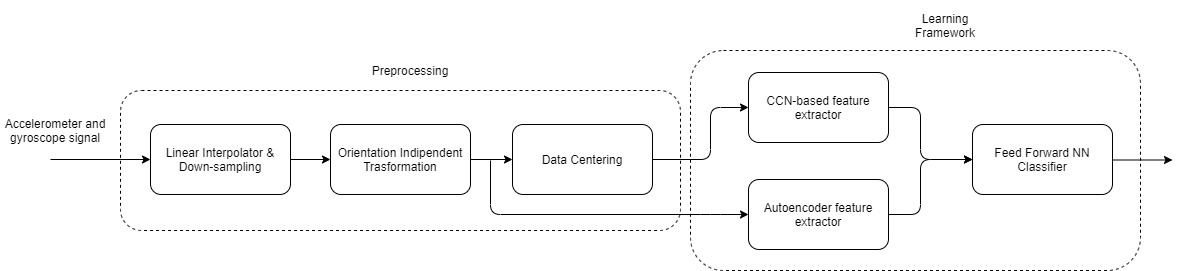
\includegraphics[width=1\textwidth]{images/processing_pipeline.jpg}
	\caption{Processing pipeline}
\end{figure*}

The task of HAR in real use case scenarios is a difficult task, and many aspects need to be considered when these applications are brought in a mobile environment. As reported in \cite{blunck2013heterogeneity} the three major types of heterogeneties which yield impairments in HAR are:
\begin{itemize}
	\item \textbf{Sensor Biases (SB)}: To keep the overall cost of a smartphone low, low costs accelerometer and gyroscope sensor are used, yielding a poor-calibrated, inaccurate an of limited granularity and range acquired signals. So, among this type of sensors we could observe differences in precision, resolution, range and also biases. Usually an initial sensors calibration are made by smartphones manufactures, but due to rotation or misalignment of the sensor to the circuit board of the final product, this could introduce errors. Furthermore, if a device experience shock, e.g falling on the ground, the sensor can be misaligned causing unwanted biases.
	\item \textbf{Sampling Rate Heterogeneity (SRH)}: Often popular smartphones vary in terms of the default and supported sampling frequencies for accelerometer and gyroscope sensor. In the dataset TODO riportare link used for this experiment for example we are dealing with smartphone where the sampling frequency varies from 50Hz to 200Hz. See Fig. TODO so the actual number of devices used in this dataset, with their corresponding sampling frequencies.
	\item \textbf{Sampling Rate Instability (SRI)}: This phenomenon is specific to a single device and regards the regularity of time span between successive measurements. Different factors could accentuate this problem, including heavy multitasking or high I/O load in the mobile device. Multitasking effect in particular is a major problem: smartphone usually prioritizes among various running tasks and doing so could extremely affects the sensor sampling of a HAR application running on the device. In our collected dataset with a 100 Hz sampling rate (which means a time-span between consecutive samples of $10ms$), for example we observe time-span ranging mainly between $3ms$ and $15ms$ with an average of $7ms$. Although in our collected dataset the smartphone was set in \textit{airplane mode} to reduce at minimum this effect. The Fig. \ref{time-span} shows the amount of different time-span present in our dataset.
\end{itemize}

\begin{figure}[h]
	\centering
	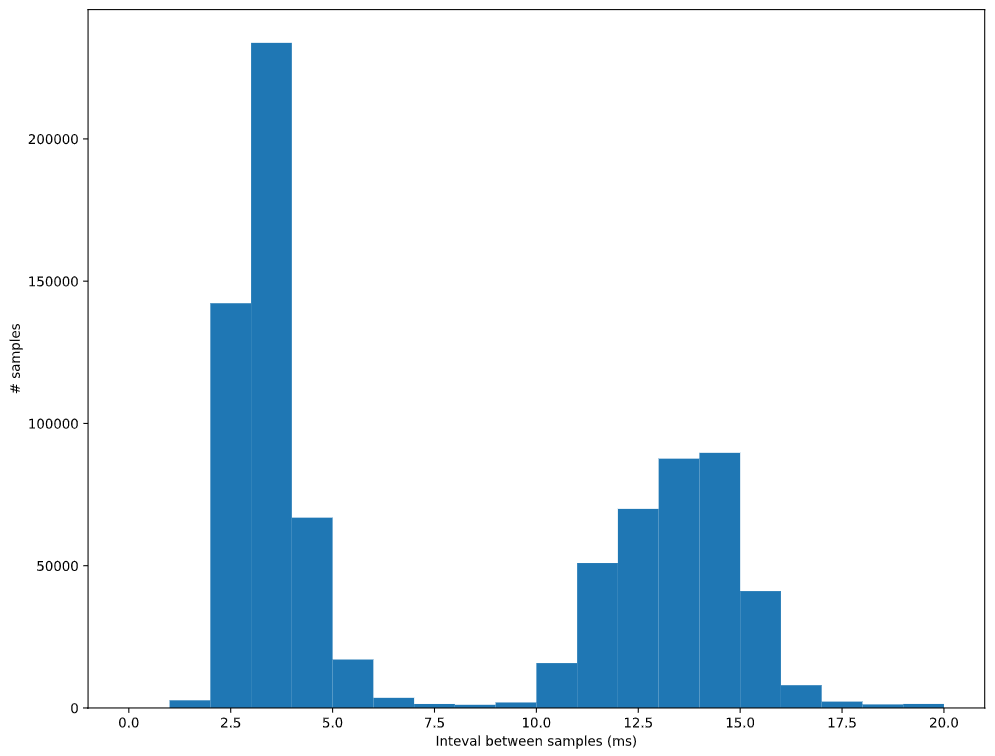
\includegraphics[width=0.4\textwidth]{images/interval_samples.png}
	\caption{Histogram of different time span between samples included in our collected dataset}
	\label{time-span}
\end{figure}

Furthermore, if we considered a real use case scenarios of a HAR mobile application we must also consider that smartphones can be positioned and oriented in different ways in human body. For example a smartphone could lay in trouser pockets (back and front) or maybe inside accessories like in a pouch or in a bag with different orientations. These different initial model settings have huge effects in prediction accuracy of an HAR predictor, especially if the model has been trained on a dataset that consist of activity measurement coming from only one fixed position and orientation of the smartphone, as is usually the case dealing with dataset collected in a controlled environment that could be found on Internet.

To tackle all these problems we decided to adopt in our pre-processing pipeline as show in Fig. TODO, 3 main blocks.

The first block called Linear Interpolator is in charge of mitigate the problems regarding the SRH and SRI as discussed previously. It main purpose is to down-sample the input data to a fixed sampling rate, in our case 50 samples/second.

The second block called Orientation Independent Transformation is used to represent data coming from different orientation of the smartphone in a rotation independent space. In this way all the signals are projected in a new space whose orientation is independent of that of the smartphone and aligned with gravity and the direction of motion. In this way an user can place his smartphone in whatever position he or she wants, mitigating the problem of different position and rotations of smartphone, as we will see in the Experiment section TODO reference.

Our last block consists of a data centering operation, applied for centering signals among y-axis that are presented only for the Covolutional Layer and not for the Autoencoder block. The reason of this choice would be clear in the section TODO. As reported in \cite{ignatov2018real}, time series centering standardize the input data, making the task for the CNN easier. Data normalization instead must be avoided because does not help in this situation since it significantly distorts time series shape, removing magnitude information which is critical for activities differentiation.

After the preprocessing pipeline we adopt a novel Learning framework. It is composed of CNN augmented with features coming from an autoencoder. As discussed in \cite{ignatov2018real} CNNs learns filters that are applied to small sub-regions of the data, and therefore they are able to capture local data pattern and their variations. Additionally, due to a small number of connections and high parallelism the amount of computations and running time of CNNs is significantly lower compared to other deep learning algorithm. This yield these model perfect for real-time HAR apps, where these models could also run in a restrict environment as one like smartphones where computation resources are limited. The only drawback of CCNs is that they fall behind in capturing global properties of the signal, and as proposed in \cite{ignatov2018real} they resolve this problem by augmenting CNNs with some basic statistical features that comprise this aspects of the data. But as opposed to what done in this latter work, where they used manual extracted features, we decided to opt for a autoencoder features extractors which can provide more robust feature. For this reason we train an auto-encoder separately on the training data and then use the encoder part to augment the CNN features used for the last classification Feed Forward Neural Network.

\section{Signals and Features}
\label{sec:model}

Parlare del nostro dataset usato Heterogenity, cioe come sono strutturati i nostri dati partenza.



\subsection{Dataset \& Meausurement Setup}
\label{subsec:dataset-measurement-setup}
Parlare di come abbiamo splittato il dataset, quindi escludendo gli utenti a e b per fare in modo di testare le performance cambiando compltamente utente.

Introduzione e spiegazione del dataset eterogeneo, preso da: riportare link. e riportare come abbiamo tirato fuori le time window con overlapping window!

Accenare dell'acquisizione di un nostro dataset alla stessa maniera, a 100 HZ in varie posizioni per testare poi anche tutto il dataset!

\subsection{Signal preprocessing}

In questo caso si va nel dettaglio (con formule e forse se neccessario anche grafici) della parte di preprocessing (parte trattegiata nel mio schema come preprocessing):

\textbf{Notation}: With $\boldsymbol{x} \in {\rm I\!R}^{n}$ we define a column vector as $\boldsymbol{x}=(x_{1}, x_{2}, ..., x_{n})^{T}$ where with superscript $^T$ we mean the transpose operator. With $\boldsymbol{||x||}$ we mean the L2-norm operator $||\x|| = (\sum_{i=1}^{n} x_{i}^{2})^{1/2}$ and with $\bar{x} = (\sum_{i=1}^{n} x_{i}) / n$ the mean of a vector. With $\boldsymbol{x} \cdot \boldsymbol{y} =\boldsymbol{x}^{T}\boldsymbol{y} $ we mean the inner product of two vectors. With $\boldsymbol{\vec{x}}$ we mean a 3D vector $\boldsymbol{\vec{x}} = (x_{1}, x_{2}, x_{3})^{T}$ and with $\boldsymbol{\hat{x}}$ the corresponding 3D versor $\boldsymbol{\hat{x}}=\boldsymbol{\vec{x}}/ ||\boldsymbol{\vec{x}}||$. For any two 3D vector $\boldsymbol{\vec{x}}$ and $\boldsymbol{\vec{y}}$ we indicate their cross-product as $\boldsymbol{\vec{x}} \times \boldsymbol{\vec{y}}$. We represent with $\boldsymbol{a_{x}}, \boldsymbol{a_{y}}, \boldsymbol{a_{z}}$ the x, y and z components of the accellerometer signal, as well as the gyroscope signal is represented with $\boldsymbol{g_{x}}, \boldsymbol{g_{y}}, \boldsymbol{g_{z}}$. We define also matrices with uppercase and bold letters. For example to define a $3 \times n$ matrix composed of 3 vectors \mbox{$\boldsymbol{x}, \boldsymbol{y}, \boldsymbol{z} \in {\rm I\!R}^{n}$} we use the notation \mbox{$\boldsymbol{M} = [\boldsymbol{x}, \boldsymbol{y}, \boldsymbol{z}]^{T}$}\\

\textbf{Linear Interpolation \& Down-sampling}\\

As described in Sec. \ref{subsec:dataset-measurement-setup}, our
dataset is composed by signals collected with different sampling rates
from many mobile phones and they are usually out of sync due to the
SRI. For this reason we apply to all signals a simple preprocessing
pipeline composed by two steps: linear interpolation and
downsampling. With linear interpolation we project signals with
different sampling frequencies, i.e 50, 100, 200 Hz, to a 50 Hz signal
which measn that we are also applying the downsampling.
Linear/nearest interpolation are usually preferred w.r.t. cubic spline
or smooth cubic spline as investigated in \cite{stisen2015smart},
because they usually mitigate the introduction of noise or
artifacts. In linear interpolation the value at time $t$ is the
piecewise-linear interpolation, i.e. the linear interpolation between
the input samples adjacent to $t$ in the sequence of input sample
timestamps. Let $(x_0, y_0)$ and $(x_1, y_1)$ be two known points, the
linear interpolant is the straight line between this points. For a
value $x$ in the interval $(x_0, x_1)$ the value $y$ along the
straight line is given from the equation of slopes
\begin{equation}
  \label{eq:linear-interpolation}
  \frac{y - y_0}{x - x_0} = \frac{y_1 - y_0}{x_1 - x_0}.
\end{equation}
It's straightforward now to see that if we need to apply linear
interpolation to a dataset of points we can calculate the \mbox{$x$-s}
given by sampling frequency we want to obtain and then apply the
formula above.

In our case the downsampling is applied in combination with linear
interpolation, but it is not always the case (see
Sec. EXPERIMENTS). It allows to standardize data at fixed sampling
frequency in order to extract time windows and feature vectors for
learning models and, above all, it reduces noise and artifacts
introduced by upsampling. Downsampling simply disregards points by
resampling the signal at a certain frequency (50 Hz in our
case). Please note that the downsample frequency should be a
sub-multiple of linear interpolation frequency.

\textbf{Orientation Indipendent Transform}\\
To project the signals acquired during an activity in a new space wich is indipendent of the rotation of the smartphone, 3 orthogonal versors need to be found. We decided to adopt the technique proposed in \cite{gadaleta2018idnet}, although many other works proposed a similar solution as in \cite{kunze2009way, henpraserttae2011accurate}. In summary we have to find these 3 orthogonal versor namely vertical versor $\boldsymbol{\hat{v}}$, horizontal versor $\boldsymbol{\hat{h}}$ and lateral versor $\boldsymbol{\hat{l}}$. As the name suggest the vertical versor is aligned with user torso pointing up, the horizontal versor is aligned with the direction of motion, pointing foraward, and the later versor tracks lateral movements and it is othogonal to the other two.

Starting with the vertical versor we need to find where the gravity vector $\boldsymbol{\vec{p}}$ ly in the original space. Although the gravity vector is a constant vector in stationary conditions, during a user activity it continuosly changes in the original cordinate system of the smartphone, therefore we are only able to consider the mean direction of the gravity within the current user activity. So, to estimate it we must considered only the acceleremoter signal: \mbox{$ \boldsymbol{\vec{p}} = (\bar{a_{x}}, \bar{a_{y}}, \bar{a_{z}})^{T}$}  and we now could find the vertical versor with \mbox{$ \boldsymbol{\hat{v}} = \boldsymbol{\vec{p}} / ||\boldsymbol{\vec{p}}|| $}

This is the first axis of our new space, and we can project the datas onto this new versor to obtain the first component axis. To do we define the acceleration matrix \mbox{$\boldsymbol{A} = [ \boldsymbol{a_{x}}, \boldsymbol{a_{y}}, \boldsymbol{a_{z}} ]^{T}$}and the gyroscope matrix \mbox{$\boldsymbol{G} = [ \boldsymbol{g_{x}}, \boldsymbol{g_{y}}, \boldsymbol{g_{z}} ]^{T} $}. Now we could project the data onto $\boldsymbol{\hat{v}}$ by:

\begin{equation}
	\label{v-axis eq}
	 \boldsymbol{a_{v}} = \boldsymbol{A} \cdot \boldsymbol{\hat{v}} ,\;\; \boldsymbol{g_{v}} = \boldsymbol{G} \cdot \boldsymbol{\hat{v}} \,.
\end{equation}

Now we have to find an horizontal plane, parallel to the floor, where the activity motion mostly occurs. To do so we have to remove the  $\boldsymbol{a_{v}}$ component from the original data. We represent the accelerometer data lying on this new plane as $\boldsymbol{M}$ representing the so called motion plane. To find $\boldsymbol{M}$ we have to: \mbox{$\boldsymbol{M} = \boldsymbol{A} - \boldsymbol{\hat{v}} \boldsymbol{a_{v}}^{T} $}

In this new plane, we could see that the direction with the largest variance of projected data, represents the main direction of motion, ie in which direction the user is currently performing the activity with respect to the current smartphone orientation. By aplying PCA \cite{rao1964use}, we are able to find the direction along which the variance of measurements is maximized. This new extracted vector it is called horizantal vector $\boldsymbol{\vec{h}}$. We now could compute the horizontal versor: \mbox{$ \boldsymbol{\hat{h}} = \boldsymbol{\vec{h}} / ||\boldsymbol{\vec{h}}|| $} and we are now able to project our data onto this second new axis by:

\begin{equation}
	\label{h-axis eq}
	\boldsymbol{a_{h}} = \boldsymbol{A} \cdot \boldsymbol{\hat{h}} , \;\; \boldsymbol{g_{h}} = \boldsymbol{G} \cdot \boldsymbol{\hat{h}} \,.
\end{equation}

To find the last axis its sufficient to apply a cross product between the two last axis found, so $ \boldsymbol{\hat{l}} = \boldsymbol{\hat{v}} \times \boldsymbol{\hat{h}} $ and the obtain our last projection of the original data into this new space by:

\begin{equation}
	\label{l-axis eq}
	\boldsymbol{a_{l}} = \boldsymbol{A} \cdot \boldsymbol{\hat{l}} , \;\; \boldsymbol{g_{l}} = \boldsymbol{G} \cdot \boldsymbol{\hat{l}} \,.
\end{equation}



Combining Eq. (\ref{v-axis eq}), Eq. (\ref{h-axis eq}) and Eq. (\ref{l-axis eq}) lead us to the final accelerometer and gyroscope trasformed vectors lying in this new orientation indipendent space that are $[\boldsymbol{a_{v}}, \boldsymbol{a_{h}}, \boldsymbol{a_{l}}]^T $ and $ [\boldsymbol{g_{v}}, \boldsymbol{g_{h}}, \boldsymbol{g_{l}}]^T $ \\

\textbf{Centering}\\

The last signal processing we perform on the input signal is data
centering. As proved in \cite{ignatov2018real} this could slightly
improve performance within a CNN based learning model because
centering the time series make the task easier for the CNN. We denote with $\x^{c}$ the centered vector of $\x$, ie
\begin{equation}
  \label{eq:centering-func}
  \x^{c} = \x - \bar{x} = (x_1-\bar{x}, x_2-\bar{x},..., x_n-\bar{x})^T.
\end{equation}
Centering is applied for each time-window only on accelerometer data, thus the new centered acceleration matrix:
\begin{equation}
  \label{eq:centering-accelerometer-data}
  \boldsymbol{A}^{c} = [\boldsymbol{a_{x}}^{c}, \boldsymbol{a_{y}}^{c}, \boldsymbol{a_{z}}^{c}]^T \,.
\end{equation}
Please note that we simply apply centering and not normalization which is common in CNN applications because normalization removes relevant information like magnitude which is critical for activities differentiation.

\subsection{Feature vector}
\label{subsec:feature-vector}

\textbf{Time windows.} When dealing with time-based signals (or
time-series in general) we must keep in mind that correlation between
samples occurs and we have to handle this useful information. However,
in the domain of LAR, even if samples can be correlated in time, the
correlation do not persist over a long period. In literature many time
window intervals were experimented CITE, CITE and they discovered that
the best time window interval is from $1$s to $2.5$s. For this reason
we adopt a sliding window approach with fixed window length of $2.5$s
with $50$\% overlap between two successive windows.

\textbf{Features}. Features are the basic elements that every machine
learning algorithm need in order to learn something. Everything fed
into a machine learning algorithm can be considered a feature, but
here we use three different type of features targetting different type
of information.

\begin{itemize}
\item \textit{Raw features}. These enables the model to
  learn directly from data and hopefully from it's shape in order
  to generalize and classify activities. Raw features are represented by
  a $6 \text{x} 125$ matrix where rows are accelerometer and gyroscope
  $x$, $y$ and $z$ dimensions while columns are samples over time.
\item \textit{Manual features}. Manual features take into account the
  statistical mode of the signal and are used in \cite{anguita2013public}
  and \cite{ignatov2018real} with great results.\footnote{FIXME: altri da citare?} We exploit
  manual features like mean, standard deviation, sum of the absolute values and
  the histogram of each input data channel computed on local
  time-windows applied only for accelerometer signal
  $\boldsymbol{a}$. As defined in \cite{ignatov2018real}, we produce a
  new basic feature vector $\boldsymbol{f_{b}} = (\bar{a_x},
  \bar{a_y}, \bar{a_z}, \sigma_{\boldsymbol{a_{x}}},
  \sigma_{\boldsymbol{a_{y}}}, \sigma_{\boldsymbol{a_{z}}},
  \tilde{a_x}, \tilde{a_y}, \tilde{a_z},
  \psi_{\boldsymbol{a_{x}}\boldsymbol{a_{y}}\boldsymbol{a_{z}}}, $ $
  \boldsymbol{h}_{\boldsymbol{a_{x}}}^T,
  \boldsymbol{h}_{\boldsymbol{a_{y}}}^T,
  \boldsymbol{h}_{\boldsymbol{a_{z}}}^T)^T$ where for a generic column
  vector $\x = (x_1, x_2,..., x_n)^T$ with \mbox{$\x^c = (x_1^c,
    x_2^c,..., x_n^c)^T$:}
  \begin{align}
    \sigma_{\x} &= \sqrt{  \frac{\sum_{i=1}^{n}(|x^c_i|)^2}{n} }\,, \\
    \tilde{x} &= \frac{\sum_{i=1}^{n}(|x^c_i|)}{n}\,, \\
    \psi_{\x\y\z} &= \frac{\sum_{i=1}^{n} \sqrt{x_i^2 + y_i^2 + z_i^2}} {n}\,,
  \end{align}
  and $\boldsymbol{h}_\x$ is column vector that sort the values of
  $\x$ into $10$ equally spaced bins along the x-axis between the
  minimum and maximum values of $\x$.\footnote{For reference, see \texttt{np.histogram} documentation.}
  This lead to a manual features vector composed of $40$ manual
  extracted features.
\item \textit{Auto-encoder features}. Auto-encoder features are
  automatically extracted from the signal. The auto-encoder as
  described in Sec. TODO is capable to compress data and learn a good
  representation of features keeping only interesting data. The code
  size we use is made up of 36 features features.
\end{itemize}

\section{Learning Framework}
\label{sec:learning_framework}

\begin{figure*}[h]
	\centering
	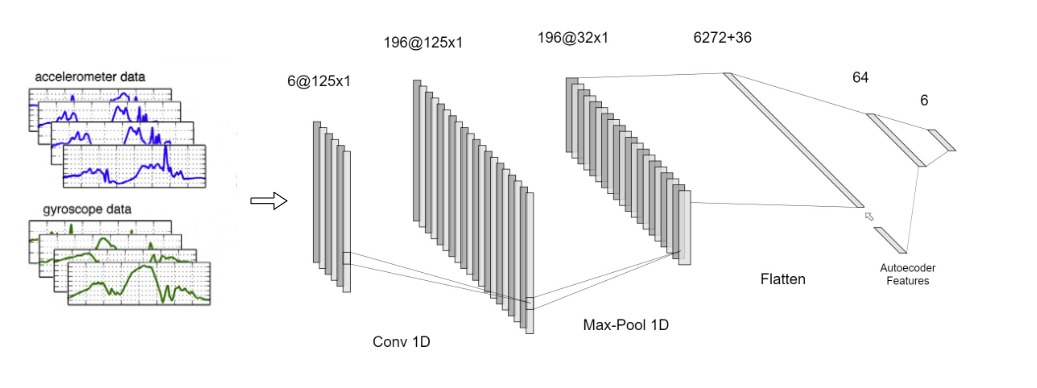
\includegraphics[width=1\textwidth]{images/full_architecture.jpg}
	\caption{Learning Framework}
	\label{fig:proposed-architecture}
\end{figure*}

In this section we will present our proposed architecture for HAR ``in
the wild'' problem. We will see how the autoencoder and the CNN are
trained, their parameters, and the optimization strategies adopted.

\subsection{Autoencoder}
\label{subsec:autoencoder}

In this section we describe the autoencoder model based on
\cite{vincent2010stacked}, \cite{gu2018locomotion} and
\cite{gao2019human}. An autoencoder is a type of artificial neural
network used to learn efficient data codings in an unsupervised
manner. The aim of an autoencoder is to learn a representation
(encoding) for a set of data by training the network to ignore signal
noise. Given $X = [ \boldsymbol{a}_v, \boldsymbol{a}_o,
  \boldsymbol{a}_l, \boldsymbol{g}_v, \boldsymbol{g}_o,
  \boldsymbol{g}_l ]^T$ as a $6\text{x}125$ matrix and $\x$ as the
column vector $750\text{x}1$ obtained by reshaping $\boldsymbol{X}$ we
can define the autoencoder in two blocks. The first block is the
encoder which is a function of the input:
\begin{equation}
  f_\theta(\x) = s(\boldsymbol{W}\x + \boldsymbol{b})
\end{equation}
where $\theta = \{ \boldsymbol{W}, \boldsymbol{b} \}$ with
$\boldsymbol{W}$ the weight matrix and $\boldsymbol{b}$ the bias
vector, while $s$ is the sigmoid activation function. We
can derive $\y = f_\theta(\x)$ as the output of this
layer. The second block is the decoder where the input is
reconstructed back starting from the code obtained by the encoder
\begin{equation}
  g_{\theta'}(\y) = s(\boldsymbol{W'}\y + \boldsymbol{b'})
\end{equation}
where $\theta' = \{ \boldsymbol{W'}, \boldsymbol{b'} \}$ are the
parameters obtained from previous step. Thus, the reconstructed input
is $\z = g_{\theta'}(\y)$. What we want to minimize is the distance
between $\x$ and $\z$ w.r.t. a distance measure with a loss function
like MSE.

The main goal of the autoencoder for this application is to extract
useful representations of input signal in few features and this is
done by looking at the autoencoder's code, i.e., the output of the
encoder block:
\begin{equation}
  \Phi_{\text{e}} = \y.
\end{equation}

The autoencoder follows the strucutre reported in
Fig. \ref{fig:encoder-structure} and is based on a Neural Network
architecture. The encoder is built with an input layer of
$6\text{x}125$ neurons reshaped as a vector $750\text{x}1$, one hidden
layer with 150 neurons and ReLU activation function, and an output
layer, i.e, the code, of $36\text{x}1$ neurons with sigmoid activation
function. The decoder replicates the same strucutre of the encoder but
reversed, where the activaction function on the output layers is the
identity.
\begin{figure}[h]
  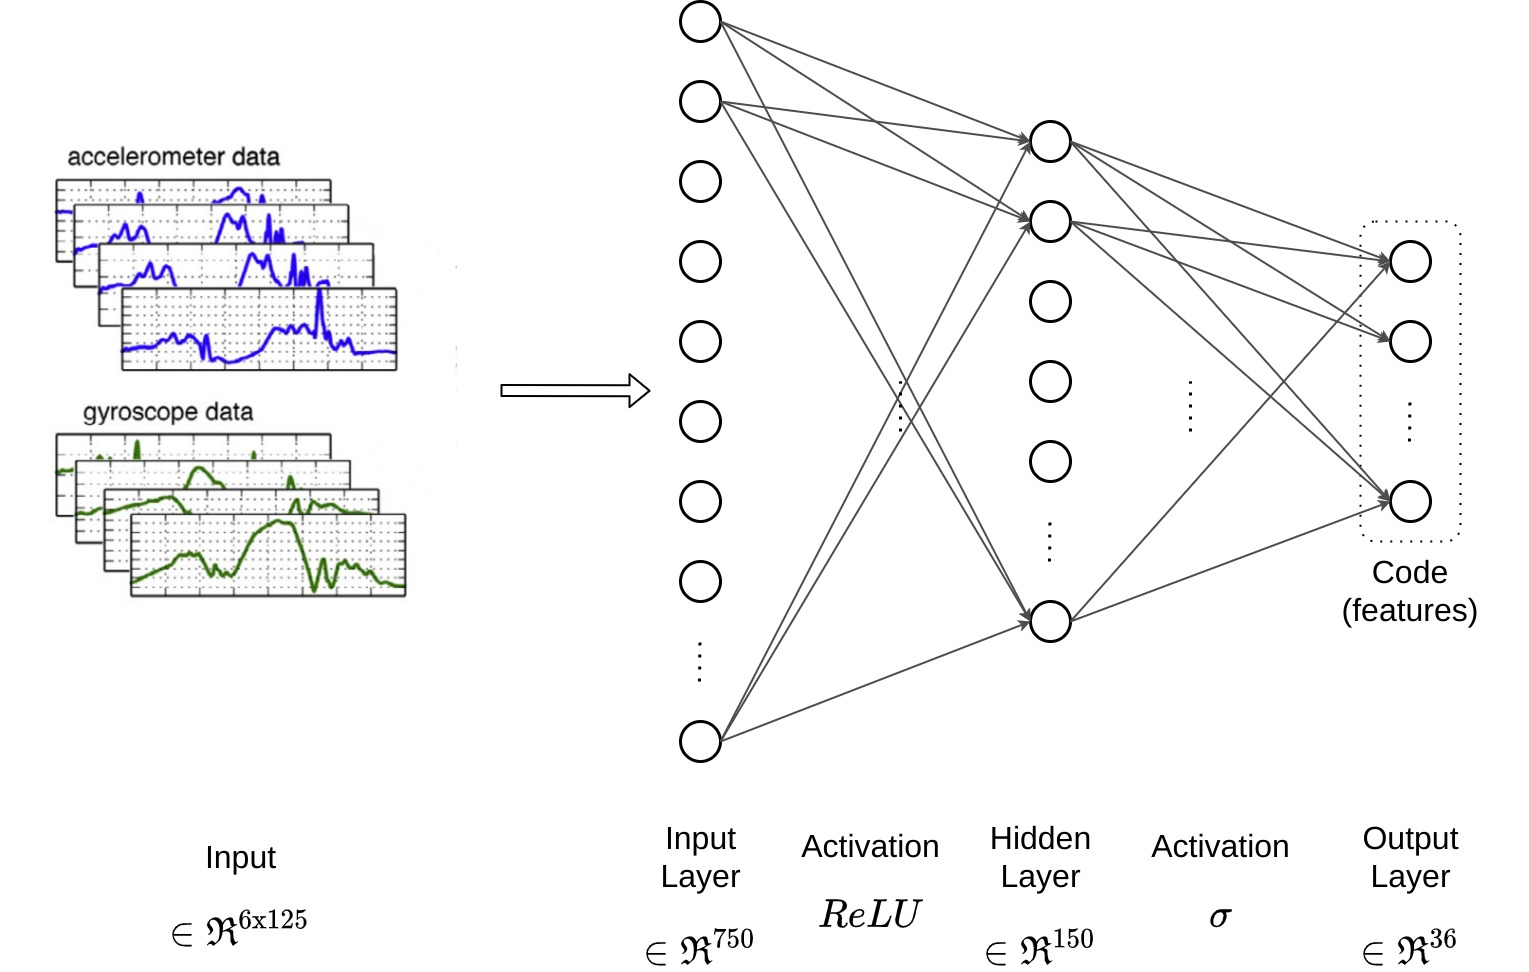
\includegraphics[width=0.5\textwidth]{images/encoder.jpg}
  \caption{(Auto)-encoder structure}
  \label{fig:encoder-structure}
\end{figure}

In order to search for best autoencoder model we tune hyperarameters
with grid search technique. Results are reported in
Tab. \ref{tab:ae-hyperparams} where values that performs well on the
validation dataset are reported in bold.
\begin{table}
  \centering
  \begin{tabular}{lp{4cm}}
    \hline
    Hyperparameter & Values \\
    \hline
    code size & \{2, 3, 4, 5, 6, 12, 18, 24, 30, \textbf{36}, 42, 48, 54, 60, 72\} \\
    batch size & \{32, \textbf{128}\} \\
    epochs & \{\textbf{150}, 200\} \\
    \hline
  \end{tabular}
  \caption{Grid-search for best hyperparameters on autoencoder}
  \label{tab:ae-hyperparams}
\end{table}
The best model used to be the one with a relatively small code
size: from 24 to 36 features which is also a good thing as we do not
want the autoencoder to learn the identity, but only to keep useful
information. The Tab. \ref{tab:ae-loss} shows how the selected
autoencoder peroforms on different scenarios.
\begin{table}
  \centering
  \begin{tabular}{lr}
    \hline
    Scenario & Loss (MSE) \\
    \hline
    heterogenity + oit + bryan & 0.747241 \\
    heterogenity + oit + bryan allpos & 0.821241 \\
    heterogenity & 0.871255 \\
    heterogenity + bryan & 10.421337 \\
    \hline
  \end{tabular}
  \caption{Autoencoder loss on different scenarios}
  \label{tab:ae-loss}
\end{table}

Even if the primary goal for this autoencoder is to automatically
extract features from signal for the main CNN model we implement also
two simple classifiers in order to directly use autoencoder's feature
and check the effectiveness of features. The two proposed model are
base on two different techniques: the first is a clustering algorithm
based on K-Nearest Neighbors (KNN) while the second is a Feed Forward
Neural Network (FFNN). The Tab. \ref{tab:ae-classifiers-accuracy}
shows KNN and FFNN accuracy for the selected model with $36$
features.\footnote{The autoencoder with $24$ features performs better
  in some cases with this two classifiers, but, again, the goal is
  to provide robust feature with CNN so we selected the model with
  lowest MSE.}
\begin{table}
  \centering
  \begin{tabular}{p{3cm}rr}
    \hline
    Scenario & KNN accuracy & FFNN accuracy \\
    \hline
    heterogenity + oit + bryan & 82.2  & 72.3 \\
    heterogenity + oit + bryan allpos &  78.9 & 68.0 \\
    heterogenity & 76.2 & 81.8 \\
    heterogenity + bryan & 27.8 & 10.3 \\
    \hline
  \end{tabular}
  \caption{NKK and FFNN accuracy ordeder by loss}
  \label{tab:ae-classifiers-accuracy}
\end{table}

\subsection{Convolutional neural network}
\label{subsec:cnn}

Parlare dell'archittettura proposta suddividendola in layer e alla fine dell'ottimizzazione adottata.

The final CNN architecture proposed in this work is shown in Fig. \ref{fig:proposed-architecture}. We decided to start with the architecture proposed in work \cite{chen2020deep} and we tried to improve it, augmenting the CNN with the encoder extracted features. CNN architecture are very powerfull when dealing with images, but they were proven to be a good features extractors also for motion data. A CNN is composed of essentially two parts: the first-one is in charge of extract features performing a dimensionality reduction over the input data, though a series of convolution and max pooling layers, and the second part of the CNN is responsible to give the final classification with usually a single fully-connected layer. Original data, collected from smartphone sensors are pre-processed according to what previously described in Sec. \ref{sec:processing_architecture}. Our input matrix presented to our CNN is the matrix \mbox{$ \boldsymbol{X} = [ \boldsymbol{a_{v}}^{c}, \boldsymbol{a_{h}}^{c}, \boldsymbol{a_{l}}^{c}, \boldsymbol{g_{v}}^{c}, \boldsymbol{g_{h}}^{c}, \boldsymbol{g_{l}}^{c}]$} wich is formed by acclerometer and gyroscopes signals, linearly interpolated at 50 samples/second  per channel with a fixed time-window of $2.5s$ with orientation independent transformation and data centering. Note that this matrix has a dimension $n \times 6$, due to the fact that TensorFlow Convolutional Layers work with input dimension of $(batch\_size, samples, channel)$.

In detail we have the following stacked layers:
\begin{itemize}
	\item \textbf{CL1}: The first convolutional is performing a Convolution 1D over the input signal. It composed of 196 filters of size ($1\times16$). Since, a convolution is defined over all the input channels, in this layer we are capturing relation among accellerometer and gyroscope data. The stride is set to 1, and the padding is configured as 'same' to have the same output dimension as te original one. After the convolution operation, we apply a $ReLU(x)=\max(0,x)$ activation function to learn non-linear correlation between signals and extract richer features. Furthermore, even if we are dealing with a small architecture, $ReLU$ activation function could prevent vanishing gradient problems, is less prone to overfitting since it induces the sparsity in the hidden units and it is extremely fast to compute, making it perfect when dealing with low computational resources.
	\item \textbf{MP1}: After the a convolutional layer, usually it is apply a max-pooling or average-pooling layer to reduce and summarize the obtained representation. We decided to use max-pool layer of size ($1\times4$), reducing by 4 times the original input shape. We call this new features representation with $ \Phi_{\text{c}} $
	\item \textbf{FC1}: After the convolutional layer and the max-pooling layer, the output of these layer is flattened into 6272 neurons. At this stage we decided to concatenate the encoder extracted features $ \boldsymbol{\Phi_{\text{e}}} $ with the Convolutional ones named $\boldsymbol{\Phi_{\text{c}}}$, creating our complete features vector $\boldsymbol{\Phi} = (\boldsymbol{\Phi_{\text{c}}}, \boldsymbol{\Phi_{\text{e}}})^T$ that is presented to the final fully-connected layer to perform the classification.
	\item \textbf{FC2-3}: These two finals layers are composed of 64 dense neuron and 6 dense neurons, respectively. These two final layers are used to perform the classification of the activity. For the FC2 we use the $ReLU$ activation function and for the final classification we apply the \textit{soft-max} activation function, which computes probability distribution over the predicted classes.
\end{itemize}

As for optimization techniques we decided to use dropout and $l_2$-regularization. The later techniques are commonly used in these types of architectures, yield a much more performance in the test set and so in generalation capabilities, preventing overfitting. We apply a dropout rate of 0.05 to the last fully-connected layer and we also apply a the $l_2$-regularization to all the fully connected layers. We have try with different hyper-parameters values for these two applied techniques, without any substantial changes in classification performance on the test set. Finally the parameters of the network are optimized using Adam CITE, a modification of stochastic gradient descent that also incorporates Momentum.


% !TEX root = template.tex

\begin{table*}[t]
	\begin{center}
		\begin{tabular}{ p{7cm}p{2cm}p{2cm}p{2cm}p{2cm} }
			\hline
			Method & Accuracy & Precision & Recall & F1-Score \\
			\hline
			CNN + No centering & 77.0 & 78.0 & 75.8 & 76.8 \\
			CNN + No centering + Manual F. & 75.6 & 76.8 & 73.9 & 75.3 \\
			CNN + Centering + Manual F. & 86.2 & 86.9 & 70.2 & 77.6 \\
			\textbf{CNN + Centering + Encoder F.} & \textbf{89.2} & \textbf{88.9} &  \textbf{86.1} & \textbf{86.1} \\
			\hline
		\end{tabular}
		\caption{\label{tab:model-performance} HD classification results with different featueres CNN augumentation and data preprocessing. The tests are made with our CNN with OIT, Data centering, 196 (1x16) filters, max-pool (1x4), 64 fully connected neurons, l2-regularization of $5e^{-5}$ and Adam learning rate of $2e^{-5}$.}
	\end{center}
\end{table*}

\section{Results}
\label{sec:results}

\subsection{Heterogenity Dataset (HD)}
\label{subsec:heterogeneity-dataset}

In this section we evaluate performances between previous works and
different model architectures and the influences of the
preprocessing techniques applied here. Similar to what was done in
\cite{ignatov2018real}, we carried out from the HD dataset some
representative users to test the model and then use the remaining ones
to train the model. In this case we selected users \textit{a} and
\textit{b} since we found that they are very representative among all
others. In fact models tend to be less precise with user \textit{a}
and more accurate with user \textit{b}. This mainly depends on the
user's style in walking, doing stairs and so on. In this way we are
able to compare results with other works that usually tend to evaluate
performances on unseen user.

In this training and test set settings, we evaluate the best
hyper-parameters for the proposed architecture model excluding OIT
preprocessing block, since this dataset was collected with a fixed
orientation. The rest of preprocessing techniques are enabled, if not
specified.

\textbf{Autoencoder.} In order to search for best autoencoder model hyper-parameters we performed a grid search. Results are
reported in Tab. \ref{tab:ae-hyperparams} where values that performs
well on the validation dataset are reported in bold. The best hyper-parameters model
used to be the one with a relatively small code size: from 24 to 36
features which is also a good thing as we do not want the autoencoder
to learn the identity, but only to keep useful information. In this
settings we get an MSE of $0.871255$.
\begin{table}[h]
  \centering
  \begin{tabular}{lp{4cm}}
    \hline
    Hyperparameter & Values \\
    \hline
    code size & \{2, 3, 4, 5, 6, 12, 18, 24, 30, \textbf{36}, 42, 48, 54, 60, 72\} \\
    batch size & \{32, \textbf{128}\} \\
    epochs & \{\textbf{150}, 200\} \\
    \hline
  \end{tabular}
  \caption{Grid-search for best hyper-parameters on autoencoder}
  \label{tab:ae-hyperparams}
\end{table}

Also, for checking autoencoder results we fine-tuned KNN parameters
with a grid search, looking for best values of distance measure and
number of neighbors. The Tab. \ref{tab:knn-grid-search} show the values.
We select the euclidean distance measure and $5$ as number of neighbors.
Due to time reasons we do not investigate further the FFNN model instead.
The obtained performances are quite satisfying: we get $76.2$\% accuracy
for KNN and $81.8$\% for FFNN.
\begin{table}[h]
  \centering
  \begin{tabular}{p{2cm}p{4.5cm}}
    \hline
    Hyper-parameters & Values \\
    \hline
    Distance measure & \{\textbf{euclidean}, manhattan, chebyshev, minkowski, standardized euclidean, mahalanobis\} \\
    Number of neighbors & \{3, 4, \textbf{5}, 6, 7, 8\} \\
    \hline
  \end{tabular}
  \caption{Grid-search for KNN classifier}
  \label{tab:knn-grid-search}
\end{table}

TODO LUCA: From the grid-search on KNN we surprisingly noticed that performances
do not vary significantly among different hyper-parameters: we get from
$76.7$\% to $80.9$\% accuracy. This may be an indication of the
maximum capability of this autoencoder model, so to obtain better
performances we have to add complexity to the model. In particular, we
noticed that KNN usually misclassify \textit{bike} activity with
\textit{no activity}, in fact \textit{bike} has only
$68$\% precision.

\textbf{CNN Network.} We fist test how number of convolutional filters in CL1 and number of dense neurons in FL2 will influence classification performances. The results obtained are presented in Tab. \ref{tab:model-selection}. We decided to choose 196 convolutional filters and 64 dense neurons thanks to its balance between accuracy and F1-Score performances, obtaining $88.9\%$ and $81.6\%$ respectively. To compare our result with that obtained in the original work \cite{stisen2015smart}, we decided to perform their \textit{Leave-one-user-out cross validation} evaluation, consisting of test the model with data from one user, and train with data from all the others in a cross validation fashion and then averaging the metrics obtained. In this evaluation setting we obtained an average F1-score of $85.8\%$, beating their best model result of nearly $10\%$ more in F1-Score metric. This prove also that using users a and b to do our evaluation is a good compromise of the real \textit{Leave-one-user-out cross validation} evaluation performances, since we obtain nearly the same results ($90.2\%$ instead of $88.9\%$ in accuracy and $85.8\%$ instead of $81.6\%$).

\begin{table}[h]
	\begin{center}
		\begin{tabular}{ p{1.8cm}p{1.7cm}p{1.7cm}p{1.7cm} }
			\hline
			CNN Filters & Dense Neurons & Accuracy & F1-Score \\
			\hline
			196 & 1024 & 84.6 & 75.3 \\
			196 & 512 & 86.1 & 75.7 \\
			\textbf{196} & \textbf{64} & \textbf{88.9} & \textbf{81.6} \\
			96 & 1024 & 82.8 & 69.9 \\
			96 & 512 & 84.4 & 73.7 \\
			96 & 64 & 89.0 & 73.0 \\
			48 & 1024 & 80.0 & 79.4 \\
			48 & 512 & 83.7 & 74.9 \\
			48 & 64 & 84.0 & 72.3 \\
			\hline
		\end{tabular}
		\caption{\label{tab:model-selection} HD classification results with data centering and manual features augmented CNN}
	\end{center}
\end{table}


To better appreciate how our preprocessing blocks affects model overall performances, we also try to disable or enable some of them. In Tab. \ref{tab:model-performance} we report our obtained results experiments. We see that augmenting the CNN with manual extracted feature when data are not centered, lead to no significant change in performances, instead when also enabling data centering preprocessing with manual features augmented CNN the model obtain nearly $10\%$ more in accuracy and precision metrics. This prove the benefits of data centering stated previously. However we were not able to reach the same performances presented in \cite{ignatov2018real}, where the authors obtained in the same exact settings an accuracy of $97.6\%$. These empirically confirm that performances of state-of-the-art models trained with one type of sensors are worse when dealing with smartphone sensors heterogeneity. Moving on, augmenting the CNN with encoder feature lead the model to better performances, meaning that encoder features are more robust that manual features, as explained previously. A confusion matrix in this latter setting is reported in Fig. \ref{fig:cnn-confusion-matrix} where we could see that the model performs nicely overall in all the considered activities, with some difficulties in distinguishing between stationary activities, stand and sit, and walk with stairs activities since probably they are very similar in sensor signals foot-prints.

\begin{figure}[h]
	\centering
	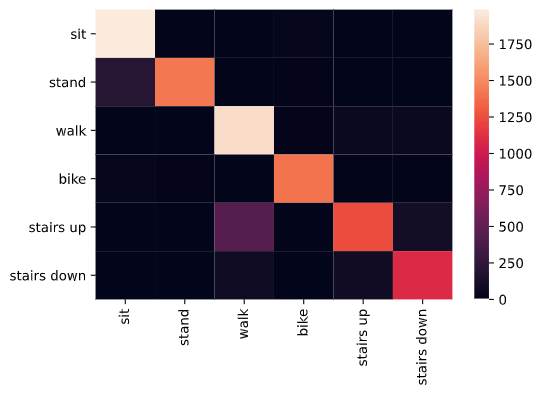
\includegraphics[width=0.5\textwidth]{images/confusion_matrix.png}
	\caption{CNN confusion matrix}
	\label{fig:cnn-confusion-matrix}
\end{figure}


\subsection{Oriented Dataset (OD)}

With these new collected dataset we want to test our model
performances in a real use case scenario, where smartphone could be
placed in different positions and orientations. In this case we
trained the model with the entire HD as training set, and then use the
OD as validation set. It is important to remember that in this case we condensed the sit and stand activities of HD into a one class no activity category, since OIT makes these two stationary activities indistinguishable from each other.

\textbf{Autoencoder.}  An interesting result, as the
Tab.~\ref{tab:ae-loss} confirms, is that OIT is a necessary operation
when dealing with HAR signals. For example, without OIT we can see
that the autoencoder trained and tested on same data goes from
$0.747241$ to $10.421337$ MSE: more than $10$x worse. Furthermore,
data from hand or pocket-up/down do not inflate the loss too
much. This is good because it indicates that autoencoder is producing
robust features.

\begin{table}[h]
  \centering
  \begin{tabular}{lr}
    \hline
    Scenario & Loss (MSE) \\
    \hline
    HD + OIT + OD validation & 0.747241 \\
    HD + OIT + OD validation (allpos) & 0.821241 \\
    HD + OD validation & 10.421337 \\
    \hline
  \end{tabular}
  \caption{Autoencoder loss on different scenarios}
  \label{tab:ae-loss}
\end{table}

The Tab. \ref{tab:knn-metrics} and \ref{tab:ffnn-metrics} show
respectively KNN and FFNN evaluation for the best autoencoder with
$36$ features and the two classifier described in
Sec. \ref{subsec:autoencoder} with hyper-parameters selected in
Sec. \ref{subsec:heterogeneity-dataset}. From this results, we can
observe that KNN is more stable and not influenced by sensor's
position/orientation w.r.t. FFNN. Also, the two models preserve order:
evaluation on \textit{pouch} position gets best results on both
models, while the worse position is \textit{hand+pocket}, as we
expected.

\begin{table}[h]
  \centering
  \begin{tabular}{lrrrr}
    \hline
    Positions & Accuracy & Precision & Recall & F1-score \\
    \hline
    Pouch & 80.1 & 86.4 & 80.7 & 79.0 \\
    Hand+Pocket & 79.5 & 83.7 & 79.5 & 79.6 \\
    All & 80.0 & 83.8 & 79.1 & 78.2 \\
    \hline
  \end{tabular}
  \caption{KNN evaluation onto OD between smartphone positions (pouch
    left/right/top/back, hand and pocket-up/down, all positions)}
  \label{tab:knn-metrics}
\end{table}

\begin{table}[h]
  \centering
  \begin{tabular}{lrrrr}
    \hline
    Positions & Accuracy & Precision & Recall & F1-score \\
    \hline
    Pouch & 74.4 & 84.7 & 74.4 & 74.8 \\
    Hand+Pocket & 67.8 & 78.0 & 67.8 & 70.0 \\
    All & 69.9 & 81.3 & 69.9 & 72.4 \\
    \hline
  \end{tabular}
  \caption{FFNN evaluation onto OD between smartphone positions (pouch
    left/right/top/back, hand and pocket-up/down, all positions)}
  \label{tab:ffnn-metrics}
\end{table}

\textbf{CNN Network.}  As reported in
Tab. \ref{tab:model-oit-performance}, we managed to get great results
also on data gathered with new sensor's position and orientation. We
noticed a performance drop of nearly $15\%$ for \textit{hand+pocket}
data, but this could be due to the CNN architecture which focus more
on the local shape and less on the real information. However, we
expected this behavior. 

\begin{table}[h]
  \begin{center}
    \begin{tabular}{p{1.8cm}rrrr}
      \hline
      Positions & Accuracy & Precision & Recall & F1-score \\
      \hline
      Pouch & 85.3 & 92.0 & 73.8 & 81.9 \\
      Hand+Pocket & 70.5 & 79.5 & 63.0 & 70.2 \\
      All & 78.0 & 84.0 & 69.0 & 75.7 \\
      \hline
    \end{tabular}
    \caption{Classification comparisons onto \textit{OD} between
      smartphone positions (pouch left/right/top/back, hand and
      pocket-up/down and all positions).}
    \label{tab:model-oit-performance}
  \end{center}
\end{table}

In conclusion, OIT revealed to be an extremely useful preprocessing
technique both for autoencoder and CNN. Without OIT, the drop for the
CNN was of nearly $45$\% for all metrics!  As Tab. confirms, combining
the power of the CNN with automatically extracted features and smart
data preprocessing could lead to good results even with new problem
settings.

\begin{table}[h]
  \begin{center}
    \begin{tabular}{lr}
      \hline
      Classifier & Accuracy \\
      \hline
      CNN + AE features & 85.3 \\
      KNN & 80.1 \\
      FFNN & 74.4 \\
      \hline
    \end{tabular}
    \caption{Comparison between KNN, FFNN and CNN classifiers onto \textit{pouch} data from OD.}
    \label{tab:classifiers-comparison}
  \end{center}
\end{table}


% !TEX root = template.tex

\section{Concluding Remarks}
\label{sec:concluding-remarks}

In this paper we proposed our solution to perform HAR 'in the wild', that could be implemented in real case scenario. Dealing with major type of heterogeneity and real use case scenario were smartphone could be positioned and oriented in any way, can be a difficult task. Using a good pre-processing pipeline, implementing linear interpolation, orientation independent transformation and Data Centering we were able to mitigate HAR impairments due to latter problems. To perform HAR, various techniques were proposed in literature: one of them very promising is the use of CNN to exploit automatic feature extraction and then compute the final classification. Augmenting CNN with more robust features like the one coming from the encoder part of an autoencoder, we were able to outperform previous results in the original work, which uses the Heterogeneity Dataset. Moreover we demonstrate that orientation independent transform is essential, allowing us to use models trained with dataset made in controlled environments, in real use case scenario with promising results. 

In future works it could be usefull to test the performance of this model with a more challenging dataset that includes: various types of persons, ie with different weights, heights, ethnicity, etc. and various type of routes where activities are performed. Moreover it could be useful to test it with subjects wearing different types of shoes and clothes. We would like also to extend the recognizable activities and also includes places were a user could be, ie be on a car, on a bus, on a train, on a plane etc. Another useful contribution, that due to lack of time we weren't able to test, is the use of open set classification techniques in which the system should reject unknown/unseen activities. Using a smartphone app, where our model was implemented, we saw that the model is constantly trying to predict the learned activities even if the user is completely doing other things with his smartphone.

With this work we learn that datasets are very important when dealing with machine learning / deep learning applications: a huge and good representative dataset of the final use case scenario onto which the model will be used, is extremely important. Moreover, pre-processing technique are very powerful and finding the right one for the project could lead to completely different results, without changing anything of the final model architecture. Furthermore, Autoencoder feature extraction could be very powerfull to augment other popular deep learning techniques.

During our project work we encounter also many problems, one of them was the bad optimization NVIDIA drivers for Ubuntu OS. The machine onto which we were performing our tests, very often crashes due to bad GPU's memory management. Also we encounter a very annoying bug using the prefetching Tensorflow dataset feature, which provide to us very different model metrics results when training multiple times the model with the same hyper parameters. After disabling that option the system provide to us comparable results when dealing with same hyper-parameters. Also we have to report that some of the paper that we red for our project were poorly written, in particular autors were not clear to present their proposed architectures. Sometimes they didn't make explicit model hyper-parameters and training settings, making it difficult to replicate their work.


\bibliography{biblio}
\bibliographystyle{ieeetr}

\end{document}


